\part{Annexe}

\chapter{Photos illustratives d'équipements informatique}

\begin{figure}[H]
	\centering
	\includegraphics[width=0.6\textwidth]{resource/img/blade}
	\caption{Trois serveurs lames (\emph{blade server} en anglais)}
\end{figure}

\begin{figure}[H]
	\centering
	\includegraphics[width=0.6\textwidth]{resource/img/netapp_c3300}
	\caption{Baie de disque NetApp C3300 contenant 14 disques durs}
	\label{netapp}
\end{figure}

\begin{figure}[H]
	\centering
	\includegraphics[width=0.6\textwidth]{resource/img/cisco-switch}
	\caption{Switch Cisco WS-C2960}
\end{figure}

\begin{figure}[H]
	\centering
	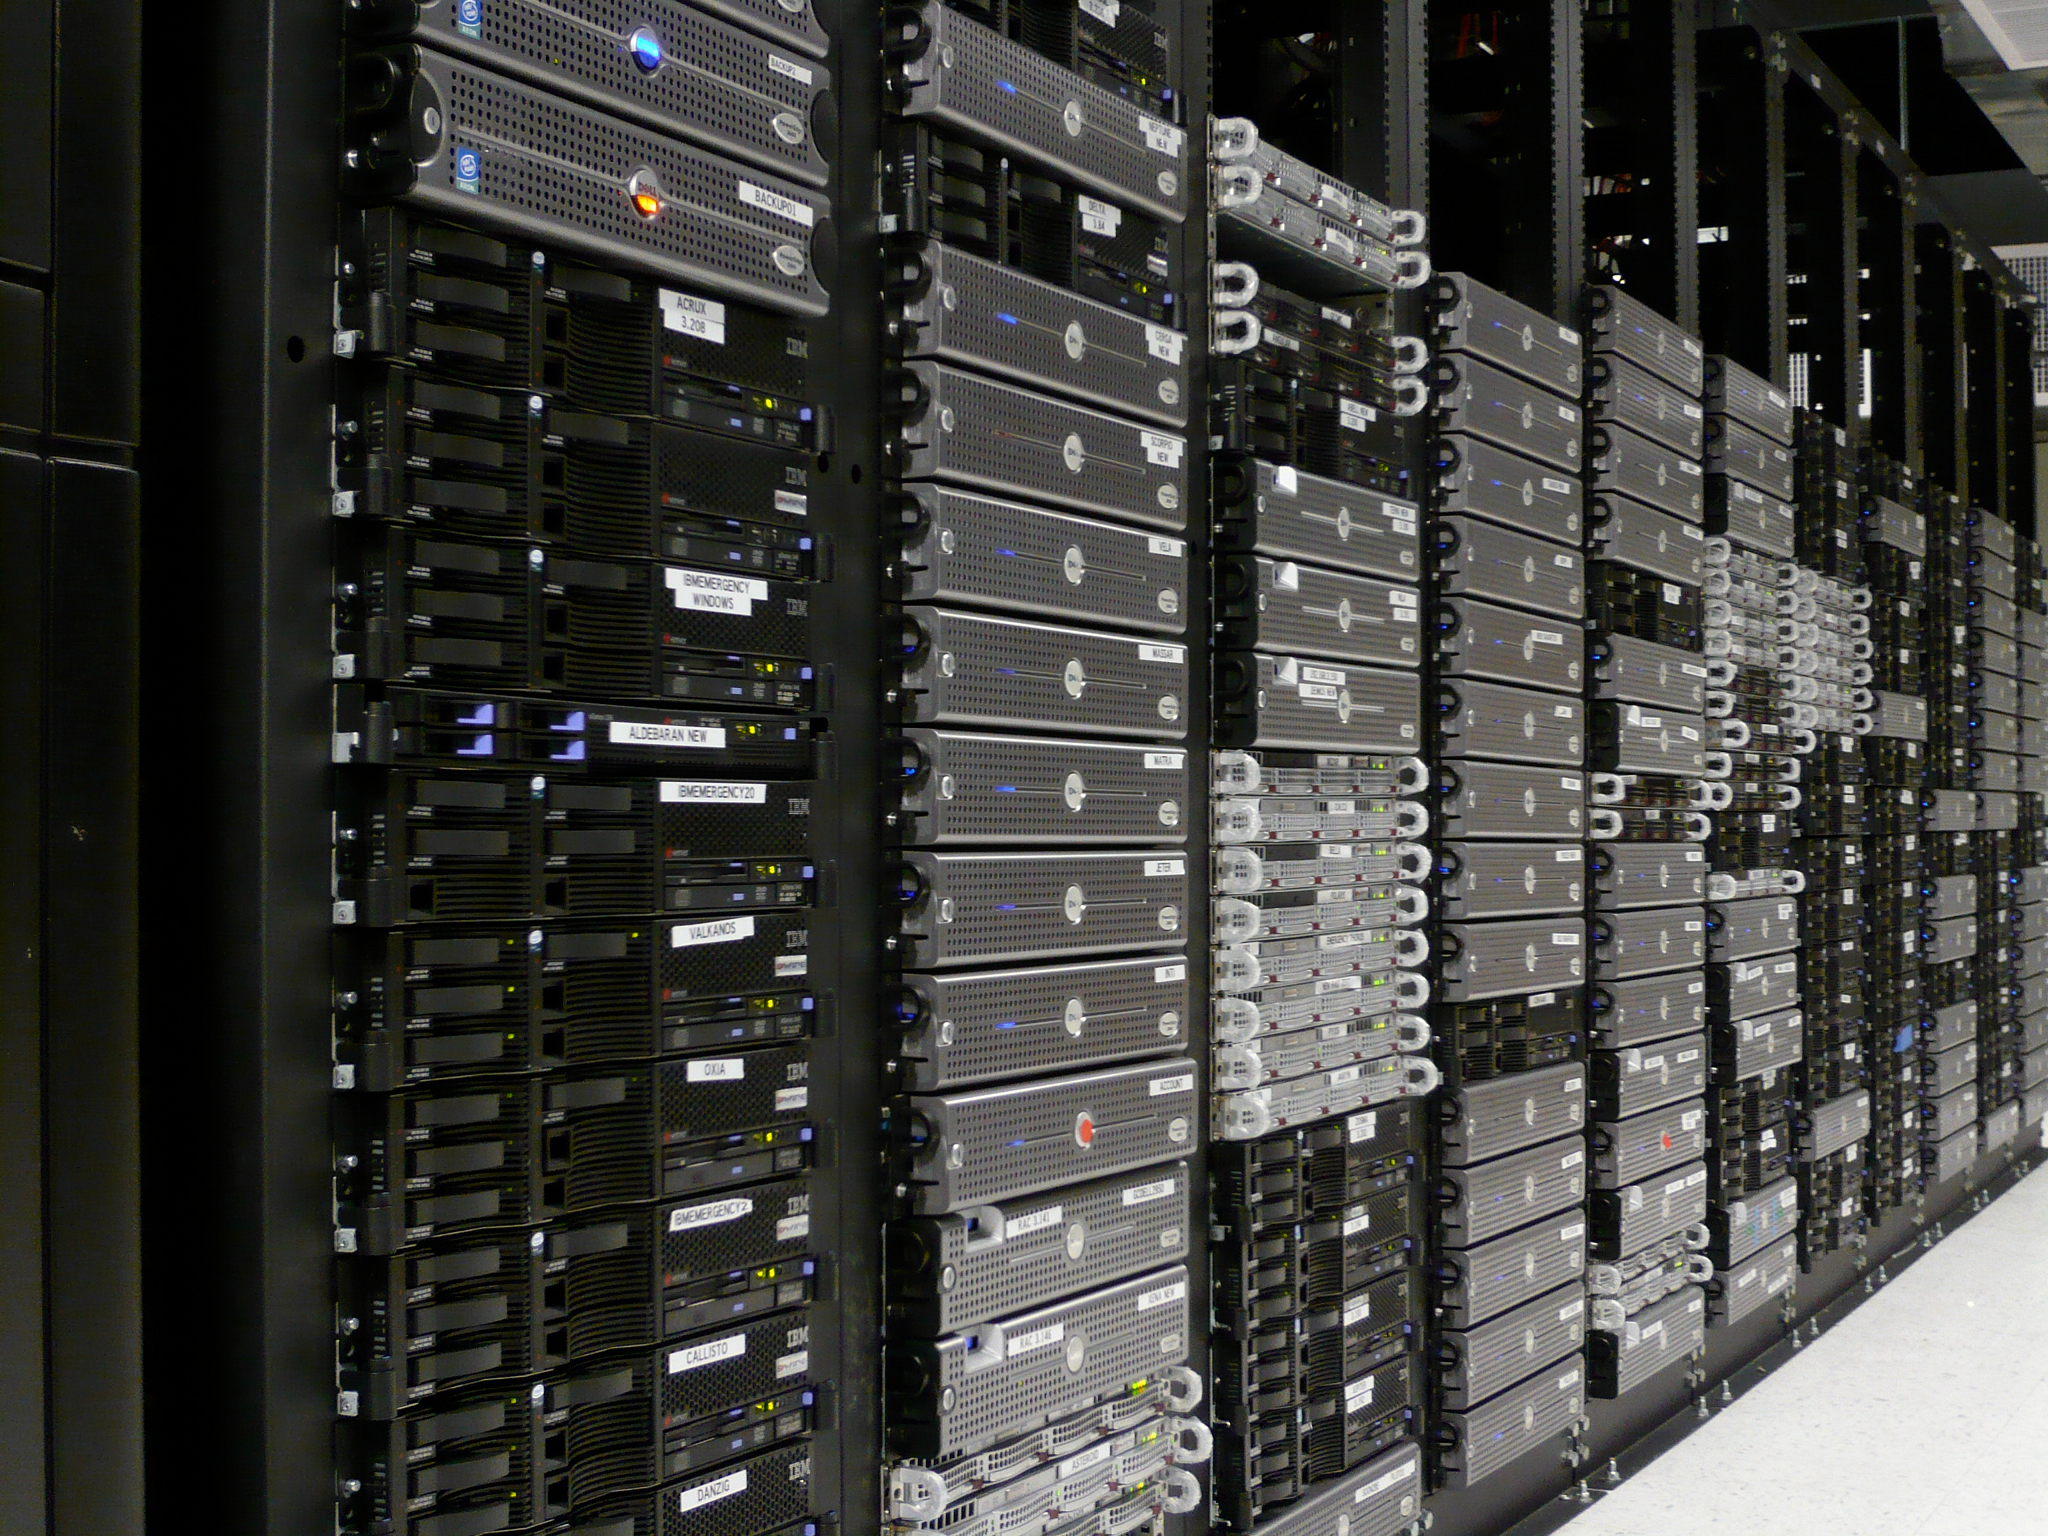
\includegraphics[width=0.6\textwidth]{resource/img/DC}
	\caption{Plusieurs baies de serveur (\emph{rack} en anglais) dans un Data Center}
	\label{datacenter}
\end{figure}

\chapter{Résumé des changement apportés à OpenNebula pour l'ajout de la gestion \emph{storage sackend}}
\label{modopennebula}
\begin{lstlisting}
 SConstruct                                     |    6 +-
 include/AuthManager.h                          |    4 +-
 include/DispatchManager.h                      |   17 ++-
 include/Image.h                                |   18 ++-
 include/ImageManager.h                         |   30 ++--
 include/ImagePool.h                            |    2 +
 include/Nebula.h                               |   26 ++-
 include/RequestManagerAllocate.h               |   39 +++-
 include/RequestManagerDelete.h                 |   18 ++
 include/RequestManagerHost.h                   |   20 ++
 include/RequestManagerImage.h                  |   27 +++
 include/RequestManagerInfo.h                   |   18 ++
 include/RequestManagerPoolInfo.h               |   18 ++
 include/RequestManagerStorageBackend.h         |   59 +++++
 include/RequestManagerUpdateTemplate.h         |   18 ++
 include/StorageBackend.h                       |  184 +++++++++++++++
 include/StorageBackendPool.h                   |   85 +++++++
 include/StorageBackendTemplate.h               |   27 +++
 include/StorageManager.h                       |  155 ++++++++++++
 include/StorageManagerDriver.h                 |   53 +++++
 include/TransferManager.h                      |   46 +++--
 include/TransferManagerDriver.h                |   89 +++++++-
 include/VirtualMachine.h                       |   17 ++-
 install.sh                                     |   34 +++-
 share/etc/oned.conf                            |   33 +++-
 share/man/SConstruct                           |    1 -
 src/acct/watch_helper.rb                       |    6 +-
 src/cli/etc/oneimage.yaml                      |    5 +
 src/cli/etc/onestoragebackend.yaml             |   50 ++++
 src/cli/one_helper.rb                          |    2 +-
 src/cli/one_helper/oneimage_helper.rb          |    8 +-
 src/cli/one_helper/onestoragebackend_helper.rb |  110 +++++++++
 src/cli/oneimage                               |   21 ++
 src/cli/onestoragebackend                      |   98 ++++++++
 src/cloud/common/CloudAuth/EC2CloudAuth.rb     |    2 -
 src/cloud/common/CloudAuth/X509CloudAuth.rb    |    3 +-
 src/dm/DispatchManagerActions.cc               |   47 ++++
 src/image/Image.cc                             |   26 ++-
 src/image/ImageManagerActions.cc               |    6 +
 src/image/ImageManagerDriver.cc                |    1 +
 src/image/ImagePool.cc                         |   37 ++-
 src/lcm/LifeCycleActions.cc                    |    1 +
 src/lcm/LifeCycleStates.cc                     |    2 -
 src/mad/MadManager.cc                          |    1 +
 src/mad/ruby/ActionManager.rb                  |   20 +-
 src/mad/ruby/StorageDriver.rb                  |  101 ++++++++
 src/mad/ruby/TransfertManagerDriver.rb         |  170 ++++++++++++++
 src/nebula/Nebula.cc                           |   31 +++-
 src/nebula/SConstruct                          |    2 +
 src/oca/ruby/OpenNebula.rb                     |    2 +
 src/oca/ruby/OpenNebula/Image.rb               |   12 +-
 src/oca/ruby/OpenNebula/Pool.rb                |   11 +-
 src/oca/ruby/OpenNebula/StorageBackend.rb      |  127 ++++++++++
 src/oca/ruby/OpenNebula/StorageBackendPool.rb  |   53 +++++
 src/oca/ruby/OpenNebula/XMLUtils.rb            |    1 -
 src/onedb/onedb                                |    6 +-
 src/onedb/onedb_backend.rb                     |   18 +-
 src/rm/Request.cc                              |    2 +
 src/rm/RequestManager.cc                       |   24 ++-
 src/rm/RequestManagerAllocate.cc               |   16 ++
 src/rm/RequestManagerImage.cc                  |   88 +++++++
 src/rm/RequestManagerStorageBackend.cc         |   69 ++++++
 src/rm/RequestManagerVirtualMachine.cc         |   18 ++-
 src/rm/SConstruct                              |    1 +
 src/sm/SConstruct                              |   12 +
 src/sm/StorageManager.cc                       |  298 ++++++++++++++++++++++++
 src/sm/StorageManagerDriver.cc                 |  228 ++++++++++++++++++
 src/sm_mad/dummy/one_sm_dummy                  |   37 +++
 src/sm_mad/dummy/one_sm_dummy.rb               |   42 ++++
 src/storagebackend/SConstruct                  |   12 +
 src/storagebackend/StorageBackend.cc           |  256 ++++++++++++++++++++
 src/storagebackend/StorageBackendPool.cc       |   87 +++++++
 src/storagebackend/test/SConstruct             |    1 +
 src/test/Nebula.cc                             |    1 +
 src/tm/TransferManager.cc                      |  131 ++++++-----
 src/tm/TransferManagerDriver.cc                |  156 ++++++++++++-
 src/tm_mad/dummy/one_tm_dummy                  |   37 +++
 src/tm_mad/dummy/one_tm_dummy.rb               |   43 ++++
 src/tm_mad/dummy/tm_dummy.conf                 |   23 --
 src/tm_mad/dummy/tm_dummy.sh                   |   19 --
 src/tm_mad/dummy/tm_dummyrc                    |   15 --
 src/tm_mad/lvm/tm_context.sh                   |    9 +-
 src/tm_mad/lvm/tm_lvmrc                        |    3 -
 src/tm_mad/shared/tm_context.sh                |   10 +-
 src/tm_mad/shared/tm_sharedrc                  |    4 -
 src/tm_mad/ssh/tm_context.sh                   |   10 +-
 src/tm_mad/ssh/tm_mv.sh                        |   17 +-
 src/tm_mad/ssh/tm_sshrc                        |    4 -
 src/tm_mad/tm_common.sh                        |   14 --
 src/vm/VirtualMachine.cc                       |    4 +
 src/vm/VirtualMachinePool.cc                   |   55 +++++
 91 files changed, 3471 insertions(+), 299 deletions(-)
\end{lstlisting}

\chapter{H2O}

\section{Résumé du code développé}

\begin{lstlisting}
 bin/h2o-archive            |  181 +++++++++++++
 bin/h2o-block              |  392 +++++++++++++++++++++++++++
 bin/h2o-cluster            |  598 +++++++++++++++++++++++++++++++++++++++++
 bin/h2o-loader             |  186 +++++++++++++
 bin/h2o-setup-db           |   22 ++
 bin/h2o-vif                |  235 ++++++++++++++++
 bin/h2o-vm                 |  529 ++++++++++++++++++++++++++++++++++++
 bin/h2ocheck               |  143 ++++++++++
 bin/h2od                   |   94 +++++++
 conf.rb                    |   11 +
 lib/cli.rb                 |  332 +++++++++++++++++++++++
 lib/dm-options.rb          |   35 +++
 lib/errors.rb              |   16 ++
 lib/lockable.rb            |   16 ++
 lib/logging.rb             |   11 +
 lib/manageable.rb          |  185 +++++++++++++
 lib/manager.rb             |   52 ++++
 lib/modules.rb             |    5 +
 lib/sshtarget.rb           |  109 ++++++++
 lib/tagable.rb             |   64 +++++
 managers/archive.rb        |   84 ++++++
 managers/block-pool.rb     |  130 +++++++++
 managers/block.rb          |  142 ++++++++++
 managers/cluster.rb        |   53 ++++
 managers/hypervisor.rb     |   94 +++++++
 managers/loader.rb         |   41 +++
 managers/vif.rb            |   99 +++++++
 managers/vm.rb             |  640 +++++++++++++++++++++++++++++++++++++++++++
 model/vm.rb                |  642 ++++++++++++++++++++++++++++++++++++++++++++
 modules/dummyblockpool.rb  |   66 +++++
 modules/dummyhypervisor.rb |   42 +++
 modules/netapp.rb          |  379 ++++++++++++++++++++++++++
 modules/xenhypervisor.rb   |  397 +++++++++++++++++++++++++++
 remote/attach-block.sh     |    3 +
 remote/pack.sh             |   23 ++
 remote/unpack.sh           |   31 +++
 templates/xmdomain.erb     |   21 ++
 tests/check.sh             |   52 ++++
 tests/cleanup-netapp.sh    |   10 +
 tests/dropshell.sh         |    4 +
 tests/reset-archivepool.sh |    4 +
 tests/reset-hyp.sh         |   10 +
 tests/reset-master.sh      |    4 +
 tests/reset-netapp.sh      |   12 +
 tests/vm-lifecycle.sh      |   59 ++++
 45 files changed, 6258 insertions(+), 0 deletions(-)
\end{lstlisting}

\section{La \emph{Command Line Interface}}
\label{CLIH2O}
\subsection{Interface de gestion de cluster}

\begin{lstlisting}
paulg@debian-pro:~/projects/h2o$ ./bin/h2o-cluster list
=>Argument Error<=
The first argument must be an action


Possible actions:
        register-hyp <cluster-id> <driver> <hostname> <ssh-user> <ssh-host>
        register-blockpool <cluster-id> <driver> <name> <target-ip> <management-ip> <management-user>
        register-cluster <name> <archive_pool_ip> <archive_pool_user>
        list-hyp [--cluster <id>] [--show-destroyed]
        list-blockpool [--cluster <id>] [--show-destroyed]
        list-cluster [--show-destroyed]
        unregister-hyp <id>
        unregister-blockpool <id>
        unregister-cluster <id>
        lock-cluster <id>
        lock-hyp <id>
        lock-blockpool <id>
        unlock-cluster <id>
        unlock-hyp <id>
        unlock-blockpool <id>
        unload-hypervisor <id>
        clear-error-cluster <id>
        clear-error-hyp <id>
        clear-error-blockpool <id>
        retry-cluster <id>
        retry-hyp <id>
        retry-blockpool <id>
        set-tag-hyp <id> [[+|-]<tag> ...]
        set-tag-blockpool <id> [[+|-]<tag> ...]
        show-hyp <id>
        show-blockpool <id>

Global optional arguments
        --raw : Print results formated for easy scripting
        --override: Disable most checks when trying to do the action
        --force: Will try harder to do the action
        --wait: Wait for the action to finish before returning
\end{lstlisting}

\subsection{Interface de gestion de VMs}

\begin{lstlisting}
paulg@debian-pro:~/projects/h2o$ ./bin/h2o-vm
=>Argument Error<=
The first argument must be an action


Possible actions:
        create <clusterId> <name>
        destroy <id>
        start <id>
        halt <id>
        reboot <id>
        mem-set <id> <size> #The memory size is in megabytes
        maxmem-set <id> <size> #The max memory size is in megabytes
        vcpu-set <id> <vcpu count>
        maxvcpu-set <id> <max vcpu count>
        show <id>
        list [--cluster <clusterId>] [--hyp <hypId>] [--show-destroyed]
        livemigrate <id> <hypervisorId>
        attach-block <id> <blockId>
        detach-block <id> <blockId>
        attach-vif <id> <vifId>
        detach-vif <id> <vifId>
        #create-if <vmId> <mac> <vlan> [--ip]... [--bandwidth] #TODO
        #destroy-if <vmId> <mac> #TODO
        pin <mvId> <hypervisorId>
        unpin <vmId>
        lock <id>
        unlock <id>
        clear-error <id>
        retry <id>
        set-tag <id> [[+|-]<tag> ...]

Global optional arguments
        --raw : Print results formated for easy scripting
        --override: Disable most checks when trying to do the action
        --force: Will try harder to do the action
        --wait: Wait for the action to finish before returning
\end{lstlisting}

\subsection{Interface de gestion des images disques (appelés blocks)}

\begin{lstlisting}
paulg@debian-pro:~/projects/h2o$ ./bin/h2o-block
=>Argument Error<=
The first argument must be an action


Possible actions:
        allocate <clusterId> <name> <size>
        clone <name> <parentBlockId>
        unpack <archiveId> <blockName> <size> <fsType:fsOptions>
        pack <blockId> <archiveName>
        deploy <id>
        list [--cluster <id>] [--show-destroyed]
        destroy <id>
        resize <id> <newSize> #The new size is in MB
        volatile <id>
        persistant <id>
        lock <id>
        unlock <id>
        clear-error <id>
        retry <id>
        set-tag <id> [[+|-]<tag> ...]

Global optional arguments
        --raw : Print results formated for easy scripting
        --override: Disable most checks when trying to do the action
        --force: Will try harder to do the action
        --wait: Wait for the action to finish before returning
\end{lstlisting}

\subsection{Interface de gestion des archives d'OS}

\begin{lstlisting}
paulg@debian-pro:~/projects/h2o$ ./bin/h2o-archive
=>Argument Error<=
The first argument must be an action


Possible actions:
        list [--cluster <id>] [--show-destroyed]
        show <id>
        upload <clusterId> <archiveName> <uri>
        (download <archiveId> <uri>)
        destroy <id>
        rename <archiveId> <newArchiveName>

Global optional arguments
        --raw : Print results formated for easy scripting
        --override: Disable most checks when trying to do the action
        --force: Will try harder to do the action
        --wait: Wait for the action to finish before returning
\end{lstlisting}

\chapter{Benchmark des I/Os disque sous Xen}

\paragraph*{}
Ces benchmarks ont été réalisés dans le but l'impact des différentes versions du noyau linux
(en DomU) sur les performances d'I/O disque des VM Xen.


\begin{figure}[H]
\centering
\subfloat[Linux 2.6.32-xen / Lecture]
	{\includegraphics[angle=-90,width=0.5\textwidth]{resource/plot/iozone-2_6_32-debian-xen-withoutcache-withoutbarrier_out_reads}}
\subfloat[Linux 2.6.32-xen / Écriture]
	{\includegraphics[angle=-90,width=0.5\textwidth]{resource/plot/iozone-2_6_32-debian-xen-withoutcache-withoutbarrier_out_writes}}
\\
\subfloat[Linux 3.1 / Lecture]
	{\includegraphics[angle=-90,width=0.5\textwidth]{resource/plot/iozone-3_1-linus-withoutcache-withoutbarrier_out_reads}}
\subfloat[Linux 3.1 / Écriture]
	{\includegraphics[angle=-90,width=0.5\textwidth]{resource/plot/iozone-3_1-linus-withoutcache-withoutbarrier_out_writes}}
\\
\subfloat[Linux 3.2 / Lecture]
	{\includegraphics[angle=-90,width=0.5\textwidth]{resource/plot/iozone-3_2-linus-withoutcache-withoutbarrier_out_reads}}
\subfloat[Linux 3.2 / Écriture]
	{\includegraphics[angle=-90,width=0.5\textwidth]{resource/plot/iozone-3_2-linus-withoutcache-withoutbarrier_out_writes}}

\caption{Cache d'écriture: \textbf{désactivé}   -   Barrière d'écriture: \textbf{désactivée}}
\end{figure}

\begin{figure}[H]
\centering
\subfloat[Linux 2.6.32-xen / Lecture]
	{\includegraphics[angle=-90,width=0.5\textwidth]{resource/plot/iozone-2_6_32-debian-xen-withcache-withoutbarrier_out_reads}}
\subfloat[Linux 2.6.32-xen / Écriture]
	{\includegraphics[angle=-90,width=0.5\textwidth]{resource/plot/iozone-2_6_32-debian-xen-withcache-withoutbarrier_out_writes}}
\\
\subfloat[Linux 3.1 / Lecture]
	{\includegraphics[angle=-90,width=0.5\textwidth]{resource/plot/iozone-3_1-linus-withcache-withoutbarrier_out_reads}}
\subfloat[Linux 3.1 / Écriture]
	{\includegraphics[angle=-90,width=0.5\textwidth]{resource/plot/iozone-3_1-linus-withcache-withoutbarrier_out_writes}}
\\
\subfloat[Linux 3.2 / Lecture]
	{\includegraphics[angle=-90,width=0.5\textwidth]{resource/plot/iozone-3_2-linus-withcache-withoutbarrier_out_reads}}
\subfloat[Linux 3.2 / Écriture]
	{\includegraphics[angle=-90,width=0.5\textwidth]{resource/plot/iozone-3_2-linus-withcache-withoutbarrier_out_writes}}

\caption{Cache d'écriture: \textbf{activé}   -   Barrière d'écriture: \textbf{désactivée}}
\end{figure}

\begin{figure}[H]
\centering
\subfloat[Linux 2.6.32-xen / Lecture]
	{\includegraphics[angle=-90,width=0.5\textwidth]{resource/plot/iozone-2_6_32-debian-xen-withcache-withbarrier_out_reads}}
\subfloat[Linux 2.6.32-xen / Écriture]
	{\includegraphics[angle=-90,width=0.5\textwidth]{resource/plot/iozone-2_6_32-debian-xen-withcache-withbarrier_out_writes}}
\\
\subfloat[Linux 3.1 / Lecture]
	{\includegraphics[angle=-90,width=0.5\textwidth]{resource/plot/iozone-3_1-linus-withcache-withbarrier_out_reads}}
\subfloat[Linux 3.1 / Écriture]
	{\includegraphics[angle=-90,width=0.5\textwidth]{resource/plot/iozone-3_1-linus-withcache-withbarrier_out_writes}}
\\
\subfloat[Linux 3.2 / Lecture]
	{\includegraphics[angle=-90,width=0.5\textwidth]{resource/plot/iozone-3_2-linus-withcache-withbarrier_out_reads}}
\subfloat[Linux 3.2 / Écriture]
	{\includegraphics[angle=-90,width=0.5\textwidth]{resource/plot/iozone-3_2-linus-withcache-withbarrier_out_writes}}

\caption{Cache d'écriture: \textbf{activé}   -   Barrière d'écriture: \textbf{activée}}
\end{figure}

\chapter{Échange de mail sur la \emph{mailing-list} d'OpenNebula}

\subsection{Mon mail}
\begin{lstlisting}
Paul Grandperrin <paul.grandperrin@alterway.fr>	 Mon, Feb 6, 2012 at 12:19 PM
To: users@lists.opennebula.org
Hi all,

I'm implementing scale-in features in OpenNebula like live memory growth/shrinking and vcpus hotplugging/hotunplugging.

You can see my git there: http://paulg.fr/gitweb/?p=one.git;a=summary;js=1
My developement branch is feature-scalein. It's still very much a WIP most of the interesting code is there and basic features are functionnal on Xen at the moment.
My dev branch is based on one-3.2 but can easily be rebased on master.

Everything is meant to eventualy hit upstream, that why I'd like to get some advices and feedback from you.

Here are my questions:

1. About VM memory scaling: Currently, AFAIK the vm.memory is used when deploying a VM to set it's initial memory and then is regularly updated via hypervisor polling.
    ATM, i'm also using this attribute to change memory size. I think it's really not the best way thing to do. I'd like to separate theses different things in separate variables.
    For exemple:
       -memory: the same as of now.
       -memory_target: the target amount of memory when scaling memory.

    I could also use VM history but I'm not very familiar with this class.

2. When scalling the number of VCPUs, should we also scale the VM's cpu share? If so, how to implement it?

3. In the case of a scalling failure (memory or vcpu), what should we do?
   -Consider the VM failed and not usable anymore? (I think it's way too strict)
   -Consider the VM still ACTIVE. However, how to inform the user about the failure (something else than writing in logs).
    And then what should we do?
       -immediatly throw a monitor request to update to the correct value?
       -Consider the worst case: if scaling down the memory => consider the old value/ if scaling up the memory, consider the new value
       -Other ideas?

Any suggestions about the code structure, writing style, naming conventions, whatever... are welcome :D

You can also see my TODO list here: http://paulg.fr/gitweb/?p=one.git;a=blob_plain;f=TODO;h=79c65a4a6eba19095a43191a75fc1e5d58d7e01a;hb=refs/heads/feature-scalein;js=1

What changed:
paulg@debian-pro:~/projects/one$ git diff one-3.2 --stat
 TODO                                      |   12 ++
 include/DispatchManager.h                 |   20 +++
 include/LifeCycleManager.h                |   20 +++-
 include/RequestManagerVirtualMachine.h    |   36 +++++
 include/VirtualMachine.h                  |   43 +++++-
 include/VirtualMachineManager.h           |   50 +++++--
 include/VirtualMachineManagerDriver.h     |   50 +++++--
 install.sh                                |    4 +-
 share/man/onevm.1                         |   60 ++++++++
 src/cli/one_helper.rb                     |    2 +-
 src/cli/one_helper/onevm_helper.rb        |   24 +++
 src/cli/onevm                             |   32 ++++
 src/dm/DispatchManagerActions.cc          |   90 +++++++++++
 src/lcm/LifeCycleActions.cc               |   68 +++++++++-
 src/lcm/LifeCycleManager.cc               |   48 ++++++
 src/lcm/LifeCycleStates.cc                |  123 +++++++++++++++
 src/mad/ruby/VirtualMachineDriver.rb      |   56 +++++--
 src/oca/ruby/OpenNebula/VirtualMachine.rb |   27 +++-
 src/rm/RequestManager.cc                  |    4 +
 src/rm/RequestManagerVirtualMachine.cc    |  105 +++++++++++++-
 src/vm/VirtualMachine.cc                  |    3 +
 src/vmm/VirtualMachineManager.cc          |  231 +++++++++++++++++++++++++++--
 src/vmm/VirtualMachineManagerDriver.cc    |   72 +++++++++-
 src/vmm_mad/dummy/one_vmm_dummy.rb        |    8 +
 src/vmm_mad/exec/one_vmm_exec.rb          |   42 +++++-
 src/vmm_mad/exec/one_vmm_sh               |    2 +-
 src/vmm_mad/remotes/xen/scale_memory      |   26 ++++
 src/vmm_mad/remotes/xen/scale_vcpu        |   26 ++++
 src/vmm_mad/remotes/xen/xenrc             |    3 +-
 29 files changed, 1204 insertions(+), 83 deletions(-)

Thank for your help,

Paul Grandperrin
\end{lstlisting}

\subsection{Le mail du \emph{Project Engineer} d'OpenNebula}
\begin{lstlisting}
Carlos Martin Sanchez <cmartin@opennebula.org>	 Wed, Feb 8, 2012 at 12:59 PM
To: Paul Grandperrin <paul.grandperrin@alterway.fr>
Cc: users@lists.opennebula.org
Hi Paul,

This is a very interesting feature. You should open a new ecosystem project [1] as soon as your code is usable, so others can test it. If you would like to see your code merged upstream once it gets to a mature enough state, make sure that whoever has to give the thumbs up in your company is aware of the License Agreement [2].

And now some quick comments to your questions:


On Mon, Feb 6, 2012 at 12:19 PM, Paul Grandperrin <paul.grandperrin@alterway.fr> wrote:
1. About VM memory scaling: Currently, AFAIK the vm.memory is used when deploying a VM to set it's initial memory and then is regularly updated via hypervisor polling.
    ATM, i'm also using this attribute to change memory size. I think it's really not the best way thing to do. I'd like to separate theses different things in separate variables.
    For exemple:
       -memory: the same as of now.
       -memory_target: the target amount of memory when scaling memory.

    I could also use VM history but I'm not very familiar with this class.


Each history entry represents a host change, so new ones are created only when the VM is deployed, migrated, or stopped + resumed. That's not the best place to log the scaling changes.

About storing the target amount of memory: VM::memory is the used memory, as reported by the polling. The memory definition, set by the user and used to create the deployment file, is taken from the MEMORY attribute of VM::obj_template. I think you should overwrite that attribute to store the target memory.

Before doing this scaling operation, you should check that the host has enough free memory. After the operation, the host share should be updated, take a look at Host::host_share, Host::add_capacity and Host::del_capacity. If you don't update the host share memory, when the VM is shutdown it will leave the host with a negative memory value.

2. When scalling the number of VCPUs, should we also scale the VM's cpu share? If so, how to implement it?

I'm not sure about the desirable behaviour. Maybe this should be decided by the user? If you are going to modify the CPU, and not only the VCPU, all the above comments about the MEMORY apply.

3. In the case of a scalling failure (memory or vcpu), what should we do?
   -Consider the VM failed and not usable anymore? (I think it's way too strict)
   -Consider the VM still ACTIVE. However, how to inform the user about the failure (something else than writing in logs).
    And then what should we do?
       -immediatly throw a monitor request to update to the correct value?
       -Consider the worst case: if scaling down the memory => consider the old value/ if scaling up the memory, consider the new value
       -Other ideas?

I've seen you are creating new LCM states. This can be very tricky, maybe you should just apply the action without moving from the RUNNING state, like the reboot action. And, if you are creating new states, at least try to keep it simple and merge those two new ones into just one. SCALING, or even a more generic... HOTPLUG?

I would always return to the RUNNING state, updating MEMORY and CPU (and Host:: host_share) in case of success.
The user will see that the operation finished, and will see if it succeeded taking a look at the VM template. You can also include an error message in the template if the operation failed.

If the scaling command returns success/failure immediately, I would not force a poll. As I said, the poll updates the used memory, not the amount set for the VM.


Regards... and good luck!

[1] http://opennebula.org/community:ecosystem
[2] http://opennebula.org/community:contribute

--
Carlos Martin, MSc
Project Engineer
OpenNebula - The Open Source Toolkit for Data Center Virtualization
www.OpenNebula.org | cmartin@opennebula.org | @OpenNebula
\end{lstlisting}


